\section{XSS: Cross-site scripting}

%-----------------------    ---------------------------------

\begin{frame}
\frametitle{¿Qué es XSS?}

\begin{itemize}
   \item Tipo de vulnerabilidad en aplicaciones web
   \item Es la más común según algunos estudios (hasta el 80\% de los ataques son XSS)
   \item Se \emph{inyecta} código en páginas web 
   \item Se utiliza para saltarse limitaciones de control de acceso (cómo \emph{same origin})
\end{itemize}

\end{frame}

%-----------------------    ---------------------------------

\begin{frame}
\frametitle{Tipos de ataques XSS}

\begin{itemize}
   \item No persistentes (en la petición HTTP o en el formulario enviado por el cliente)
   \item Persistentes (cuando el código proviene del servidor servidor)
   \item DOM-based XSS (no interviene el servidor)
\end{itemize}



Para evitarlos:

\begin{itemize}
  \item Validar cualquier tipo de datos enviados por los usuarios (i.e., \emph{sanitizing} -limpiar- la petición)
\end{itemize}

\end{frame}


%-----------------------    ---------------------------------

\begin{frame}
\frametitle{Ejemplo de ataque XSS: No persistente}

\begin{center}
  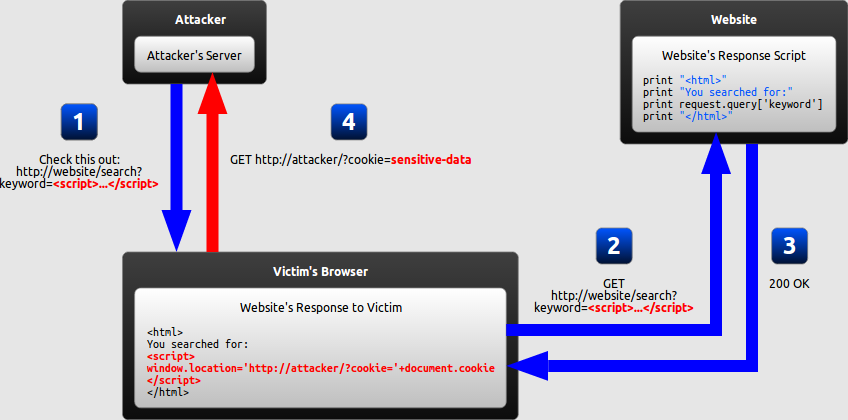
\includegraphics[width=12cm]{figs/reflected-xss}
\end{center}


\begin{flushright}
{\tiny
Source: http://excess-xss.com/reflected-xss.png
}
\end{flushright}

\end{frame}

%-----------------------    ---------------------------------

\begin{frame}
\frametitle{Ejemplo de ataque XSS: Persistente}

\begin{center}
  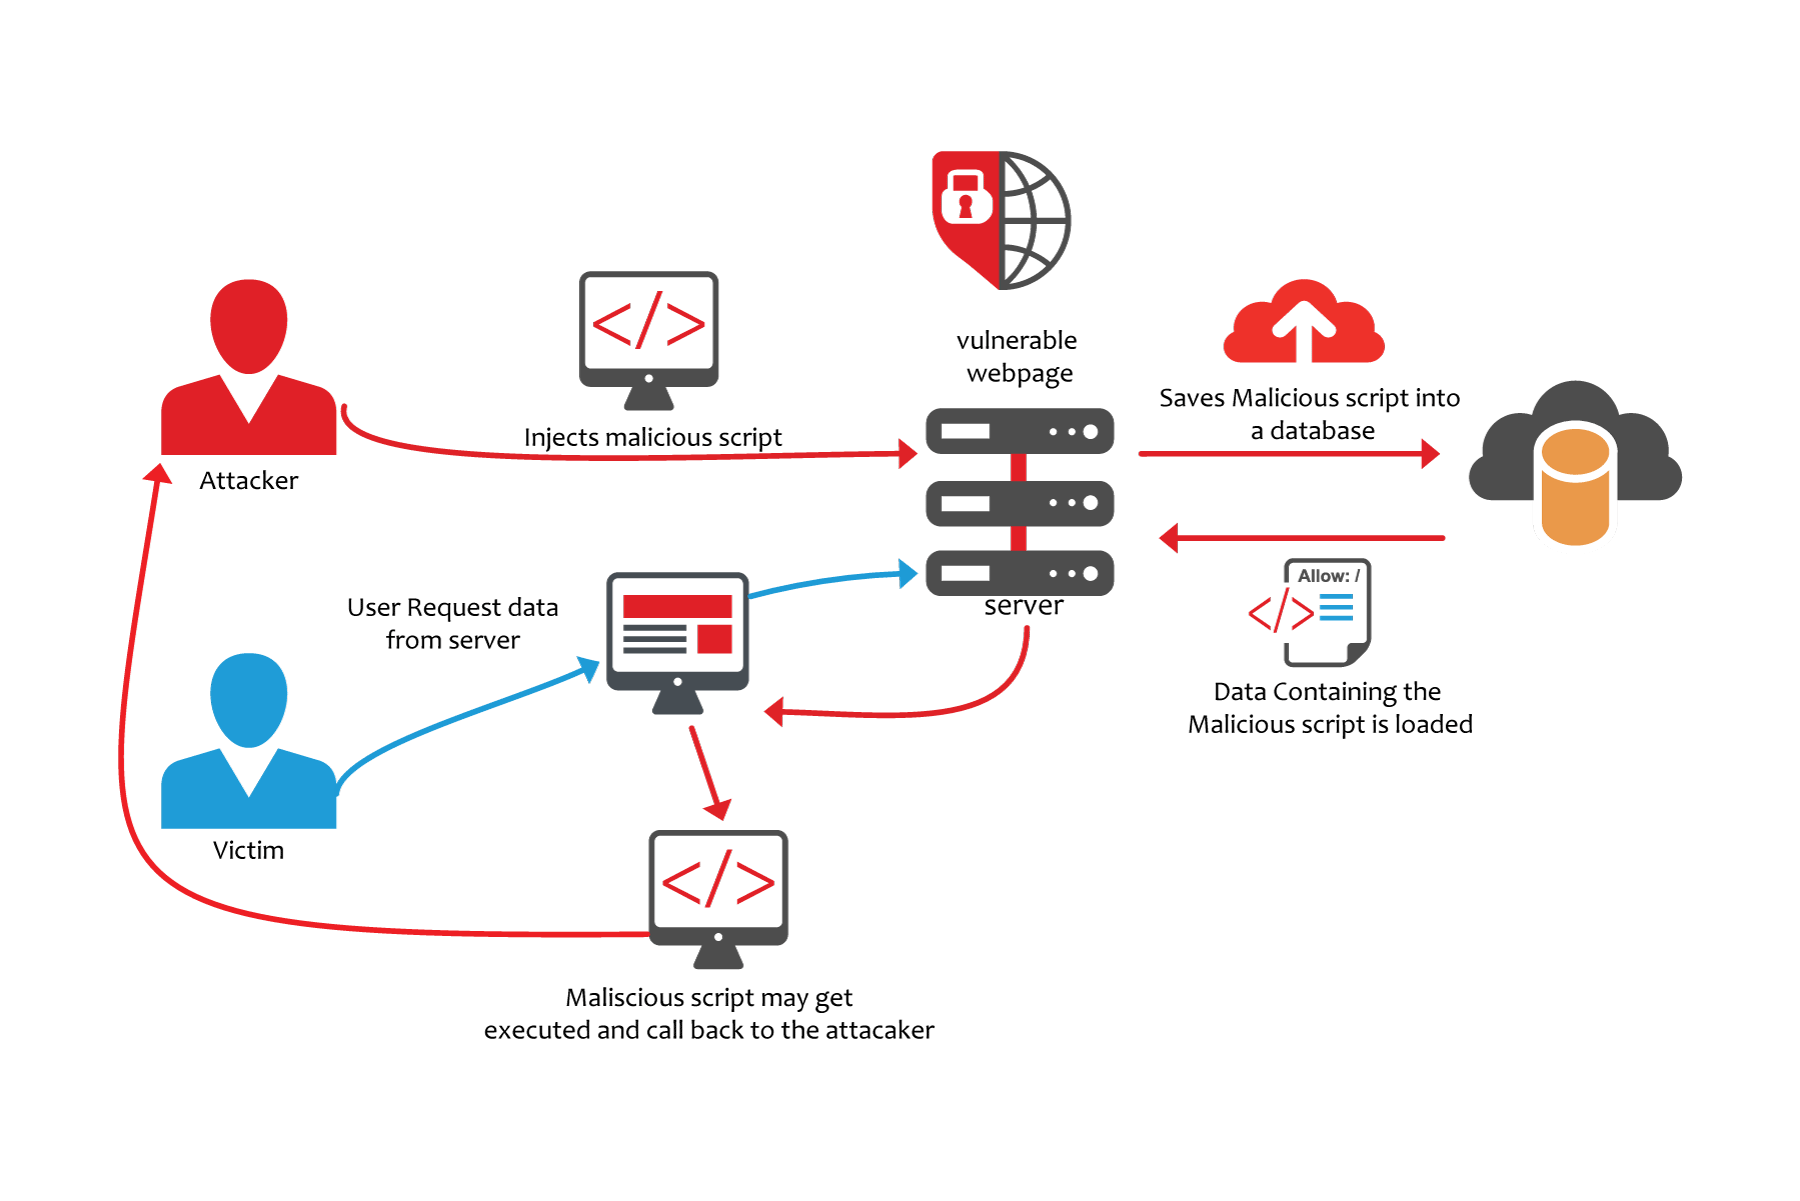
\includegraphics[width=10.5cm]{figs/Diagram-Describing-Blind-XSS-Attack}
\end{center}


\begin{flushright}
{\tiny
Source: http://www.acunetix.com/wp-content/uploads/2013/08/Diagram-Describing-Blind-XSS-Attack.gif
}
\end{flushright}

\end{frame}


%-----------------------    ---------------------------------

\begin{frame}
\frametitle{Ejemplo de ataque XSS: DOM-based}

\begin{center}
  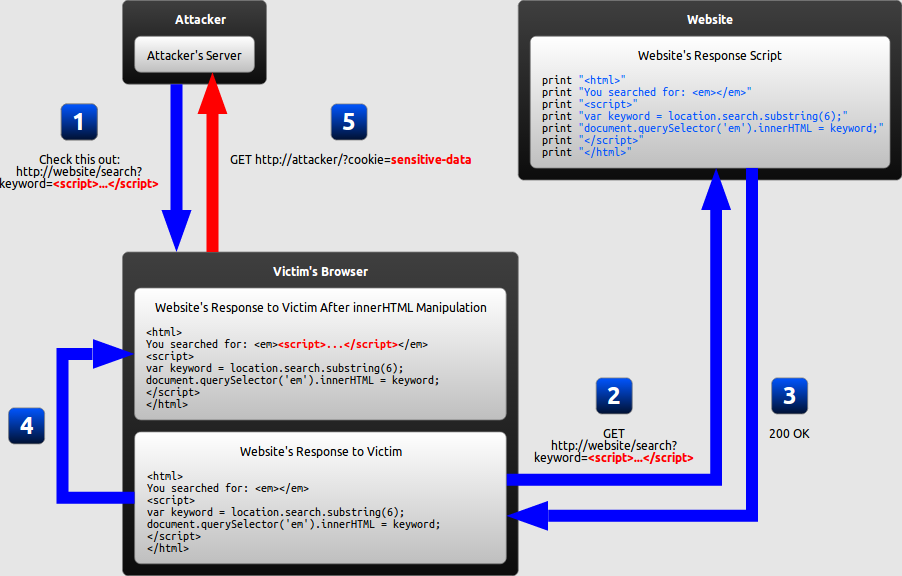
\includegraphics[width=11cm]{figs/dom-based-xss}
\end{center}


\begin{flushright}
{\tiny
Source: http://excess-xss.com/dom-based-xss.png
}
\end{flushright}

\end{frame}
